\section{Privacy and Integrity of Data Storage}
La comunità di ricerca è stata molto attiva e ha prodotto diversi contributi e avanzamenti:
\begin{itemize}
    \item soluzioni per proteggere la confidenzialità dei dati salvati
    \item indicizzazione che supporta differenti tipi di query
    \item valutazione di esposizione delle inferenze
    \item integrità dei dati
    \item accesso selettivo 
\end{itemize}
Le soluzioni per proteggere i dati possono essere basate su:
\begin{itemize}
    \item criptazione
    \item criptazione e frammentazione
    \item frammentazione
\end{itemize}

\subsection{Criptazione}
Il server può essere \textbf{honest-but-curious} cioè protegge l'integrità ma non è affidabile sulla protezione della sensibilità. La confidenzialità può essere protetta aggiungendo uno strato di criptazione sui dati sensibili (e per ragioni di performance, la criptazione, è fatta a livello di tuple):
\begin{itemize}
    \item a livello di tabella, ma se dovessi fare una query dovrei decriptare tutto
    \item a livello di tuple, ma non potrei fare proiezioni
    \item a livello di attibuto, ma non potrei fare selezioni
    \item a livello di cella, richiede tante operazioni  di criptazione e decriptazione
\end{itemize}
Per ragioni di confidenzialità i CSPs che immagazzinano dati non posso decriptarli per processarli o per accederci. Per questo abbiamo bisogno di un meccanismo che ci permetta di accedere a questi dati che sia effettivo ed efficiente e che non dia la possibilità di fare inferenze.\\
Esistono diversi approcci:
\begin{itemize}
    \item \textbf{Keyword search}: ricerca di stringhe sui dati criptati, non è una query ma string matching. Il server non deve decriptare.
    \item \textbf{Homomorphic encryption}: si eseguono le operazioni sui dati criptati. Questo è molto costoso.
    \begin{itemize}
        \item Fully Homomorphic: operazione sul criptato ha lo stesso risultato che l'operazione fatta sui dati in chiaro e poi criptati
        \item Addition and Multiplication Homomorphic: rispetto ad addizione e moltiplicazione
        \item Order Preserving Homomorphic: posso valutare se è maggiore, minore o uguale
        \item Deterministic Homomorphic: mi dice se ho corrispondenza 1 a 1 
        \item Random Homomorphic: non mi dice nulla
    \end{itemize}
    \item \textbf{Encryption Schemas}: ogni colonna può essere criptata con uno schema diverso a seconda di determinate condizioni che vengono valutate su di esse
    \item \textbf{Onion Encryption}: cripto i dati a cipolla dove ogni livello supporta l'esecuzione di specifiche operazioni SQL. Il problema con questo metodo è che quando la "cipolla è pelata", rimane pelata; se il criptato è order preserving allora la crittografia fa leak dell’ordine.
    \item \textbf{Indexes}: vengono allegati dei metadati ai dati e sono utili per fare le query. Ad esempio il WHERE della query non è valutato sul criptato ma sugli indici associati. 
\end{itemize}

\subsubsection{Criptazione e Indici}
Come è fatta una tabella criptata indicizzata?
\begin{center}
    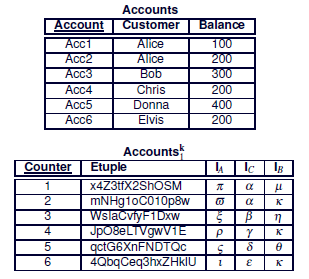
\includegraphics[scale=0.6]{img/tabind.png}
\end{center}
La tupla viene criptata interamente dando come risultato la stringa contenuta in Etuple. Per ciascun attributo sul quale devo valutare delle condizioni, specifico dei metadati (nel nostro caso le colonne Account, Customer e Balance diventano gli indici contenuti nelle colonne\(I_A, I_C, I_B\)).\\
Come funziona questo processo?
\begin{center}
    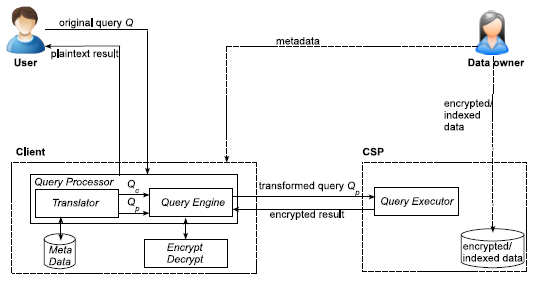
\includegraphics[scale=0.6]{img/queryprocess.png}
\end{center}
Il data owner:
\begin{enumerate}
    \item cripta i dati
    \item li indicizza
    \item li memorizza sul server
\end{enumerate}
L'utente per accedere ai dati deve per forza passare a un Client trusted:
\begin{enumerate}
    \item fa una query
    \item la query viene tradotta in una query che opera su gli indici
    \item prende il risultato
    \item decripta il risultato
    \item fa una post computazione
    \item ritorna i risultati all'utente
\end{enumerate}
Come indici possiamo utilizzare diversi valori:
\begin{itemize}
    \item \textbf{Direct (1:1)}: uso un valore vero o una codifica del valore vero. In questo caso ad un indice corrisponde un dato specifico. Vantaggi: approccio semplice e preciso per query di uguaglianza (riesco a valutare più precisamente le query). Svantaggi: preserva la distinguibilità dei valori reali e quindi soggetto ad attacchi di inferenza (in particolare attacchi di frequenza). Esempio:
    \begin{center}
        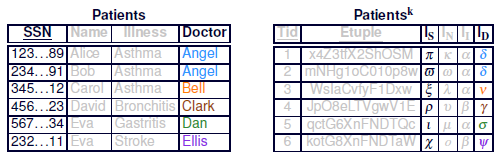
\includegraphics[scale=0.6]{img/dirind.png}
    \end{center}
    Angel è più esposto perchè è l'unico che compare due volte
    \item \textbf{Bucket (n:1)}: inizio ad avere collisioni dove valori diversi si mappano allo stesso valore indicizzato. Vantaggi: supporta ancora query di uguaglianza , la collisione rimuove la distinguibilità. Svantaggi: i risultati possono contenere risultati che io non ho richiesto e quindi devo effettuare del post processing per filtrare solo le tuple che mi servono, siamo ancora vulnerabili a attacchi di inferenza (frequenza)
    \begin{center}
        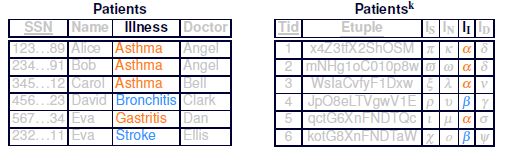
\includegraphics[scale=0.6]{img/bucketind.png}
    \end{center}
    Sapendo le reali frequenze posso capire che l'asma non è in beta.
    \item \textbf{Flattened (1:n)}: un valore in chiaro può essere mappato a più indici. Vantaggi: riduce la possibilità di ricevere attacchi di inferenza. Svantaggi: rimane vulnerabile all'osservazione dinamica (se faccio le query chiedendo di Eva mi ritorneranno tutti gli indici e so che saranno associati ad Eva)
    \begin{center}
        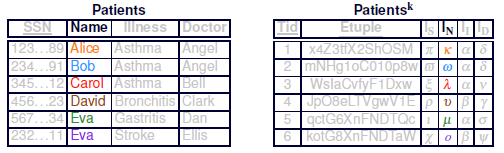
\includegraphics[scale=0.6]{img/flattind.png}
    \end{center}
    Eva era doppia e l'ho mappata con due indici diversi. 
\end{itemize}

\subsubsection{Partition-based index}
Consideriamo un arbitrario attributo col testo in chiaro \(A_i\) in uno schema relazionale R con dominio \(D_i\). \(D_i\) è partizionato in un numero di sottoinsiemi non sovrapponibili, chiamate partizioni, che contengono valori contigui. \\
Data una tupla t in r, il valore dell'attributo \(A_i\) per t appartiene ad una partizione: la funzione \(ident_{R.A_i}(p_j)\) assegna ad ogni partizione \(p_j\) di attributi \(A_i\) in R un identificatore.\\
Il valore che corrisponde all'indice è l'unico valore associato con la partizione a cui l'attributo \(t[A_i]\) appartiene: \[Map_{R.A_i}(v) = ident_{R.A_i}(p_j)\]
dove \(p_j\) è la partizione che contiene v.\\
Map può essere random o order-preserving (l'ordine degli indici è uguale a quello sulle tuple in chiaro).
\begin{center}
    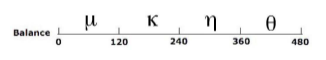
\includegraphics[scale=0.7]{img/partbased.png}
\end{center}
In questo esempio:
\begin{itemize}
    \item \(Map_{Balance}(100) = \mu \)
    \item \(Map_{Balance}(200) = \kappa \)
    \item \(Map_{Balance}(300) = \eta \)
    \item \(Map_{Balance}(400) = \theta \)
\end{itemize}
Questo metodo supporta le query dove le condizioni sono formule booleane nella forma: 
\begin{itemize}
    \item Attribute op Value
    \item Attribute op Attribute
\end{itemize}
dove op include \(\{=, <, >, \leq, \geq\}\). Più nello specifico:
\begin{itemize}
    \item \textbf{\(A_i = v\)}, il mapping è definito come \[ Map_{cond}(A_i = v) \Longrightarrow I_i = Map_{A_i}(v) \]
    Nell'esempio \( Map_{cond}(Balance = 100) \Longrightarrow I_B = Map_{Balance}(100) = \mu \)
    \item \textbf{\(A_i < v\)}, il mapping dipende dalla funzione \(Map_{A_i}\) se è random o order-preserving:
    \begin{itemize}
        \item se è order-preserving: \(Map_{cond}(A_i < v) \Longrightarrow I_i \leq Map_{A_i}(v) \)
        \item se è random: si controlla se l'attributo appartiene in una delle partizioni che potrebbe contenere il valore cercato:\\ \(Map_{cond}(A_i < v) \Longrightarrow I_i \in Map_{A_i}^<(v) \)
    \end{itemize}
    \item \textbf{\(A_i > v\)} è simmetrico rispetto al punto precedente
    \item \textbf{\(A_i = A_j\)} la traduzione è fatta considerando tutte le possibili coppie di partizioni che si sovrappongono. Formalmente
    \[Map_{cond}(A_i = A_j) \Longrightarrow \lor_\phi(I_i = ident_{A_i}(p_k) \land I_j = ident_{A_j}(p_l)) \]
    dove \(\phi\) è \(p_k \in\) partion(\(A_i\)), \(p_l \in\) partion(\(A_j\)), \(p_k \cap p_l \neq \emptyset\)
    \begin{center}
        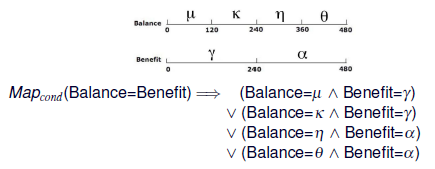
\includegraphics[scale=0.7]{img/mapcond.png}
    \end{center}
    \item \textbf{\(A_i < A_j\)} il mapping dipende dalle funzioni \(Map_{A_i}\) e \(Map_{A_j}\) se sono order preserving o meno
    \begin{itemize}
        \item \(Map_{A_j}\) è order-preserving: la traduzione considera tutte le partizioni di \(A_i\) e identifica tutte le partizioni di \(A_j\) che soddisfano la condizione di ordine. Formalmente:
        \[ Map_{cond}(A_i < A_j) \Longrightarrow \lor_{p \in partition(A_i)} (I_i=ident_{A_i}(p) \land I_j \geq Map_{A_j}(p.low)) \]
        
        \item \(Map_{A_i}\) è order-preserving: simmetrico al caso precedente
        \[ Map_{cond}(A_i < A_j) \Longrightarrow \lor_{p \in partition(A_j)} (I_j=ident_{A_j}(p) \land I_i \leq Map_{A_i}(p.high)) \]
        
        \item  \(Map_{A_i}\) e \(Map_{A_j}\) sono entrambe order-preserving:
        \[ Map_{cond}(A_i < A_j) \Longrightarrow \lor_\phi (Map_{A_i}(p_k.low)) \leq Map_{A_j}(p_l.high)) \]
        dove \(\phi\) è \(p_k \in partition(A_i)\) e \(p_l \in partition(A_j)\)
        
        \item \(Map_{A_i}\) e \(Map_{A_j}\) sono entrambe random: la traduzione considera tutte le coppie di partizioni di \(A_i\) e \(A_j\) che soddisfano la condizione. Formalmente:
        \[ Map_{cond}(A_i < A_j) \Longrightarrow \lor_\phi  (I_i = ident_{A_i}(p_k) \land I_j = ident_{A_j}(p_l)) \]
        dove \(\phi\) è \(p_k \in partition(A_i)\), \(p_l \in partition(A_j)\) e \(p_l.high \geq p_k.low\)
        
    \end{itemize}
\end{itemize}
Ogni query Q nel database viene tradotta in:
\begin{itemize}
    \item una query per il server \(Q_s\) 
    \item una per il client \(Q_c\) 
\end{itemize}. 
La query per il server \(Q_s\) opera sugli indici quindi è la traduzione delle query per il client usando le regole viste sopra. \\
Quando il risultato arriva al client viene decriptato e il client può eseguire la propria query, rimuovendo le parti che non servono e che sono finite lì a causa della collisione tra indici. \\
L’importante è che il risultato sia completo: meglio avere più tuple piuttosto che meno. \\
Altra cosa a cui bisogna stare attenti: se il server ha anche funzioni di computazione devo fare in modo che parte della computazione sia a carico suo, non avrebbe senso portarsi sul client tutta una parte di db e poi fare tutta la computazione.\\
Vediamo un esempio:
\begin{center}
    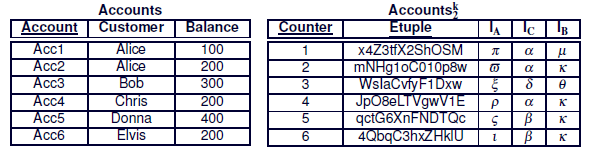
\includegraphics[scale=0.6]{img/querytrans.png}
\end{center}
La query originale avrà una struttura simile:
\begin{minted}{sql}
    SELECT *
    FROM Accounts
    WHERE Balance = 200
\end{minted}
e andrà ad ottenere come risultati Acc2, Acc4, Acc6.\\
La query tradotta \(Q_s\) invece avrà una struttura simile:
\begin{minted}{sql}
    SELECT Etuple
    FROM Accounts2k
    WHERE Ib = k
\end{minted}
che otterrà come risultati le righe 2, 4, 5, 6.\\
Ovviamente in questa query ci sono risultati che io non vorrei, quindi lato del DBMS (client) devo ripulire questi risultati sporchi e fare un'ultima query:
\begin{minted}{sql}
    SELECT *
    FROM Decrypt(Qs, Key)
    WHERE balance = 200
\end{minted}
che darà come risultato le righe Acc2, Acc4, Acc6.

\subsubsection{Hash-based index}
Basato sul concetto di one-way hash function.\\
Per ogni attributo \(A_i\) c'è una funzione di hash \(h : D_i \righarrow B_i\) dove \(B_i\) è il dominio dell'index \(I_i\) associato ad \(A_i\).\\
Data una tupla con il testo in chiaro t in r, il valore dell'indice che corrisponde a \(t[A_i]\) è \(h(t[A_i])\)\\
Le proprietà importanti di ogni funzione sicura di hash h sono:
\begin{itemize}
    \item \textbf{determinismo}: \( \forall x,y \in D_i: x = y \Longrightarrow h(x) = h(y) \)
    \item \textbf{collisione}: dati due valori \( x,y \in D_i\) con \(x \neq y\) possiamo avere che \(h(x) = h(y)\)
    \item \textbf{strong mixing}: dai due valori vicini ma distinti \(x,y (|x - y| < \epsilon) \) scelto a caso in \(D_i\) la distribuzione della probabilità discreta della differenza \(h(x) - h(y)\) è uniforme
\end{itemize}

\begin{center}
    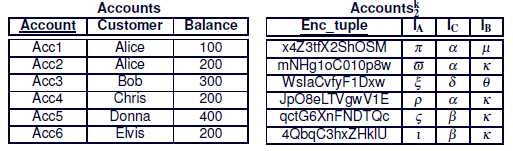
\includegraphics[scale=0.6]{img/hashindex.png}
\end{center}
Abbiamo che:\\
\(h_c(Alice) = h_c(Chris) = \alpha \) \\
\(h_c(Donna) = h_c(Elvis) = \beta \) \\
\(h_c(Bob) = \delta \) \\
\(h_b(200) = h_b(400) = \kappa \) \\
...\\
Questo metodo di indexing supporta le query dove le condizioni sono formule booleane dei termini, nella forma:
\begin{itemize}
    \item Attribute = Value
    \item Attribute1 = Attribute2, se Attribute1 e Attribute2 sono indicizzati con la stessa funzione di hashing
\end{itemize}
Non supporta query di range a causa dello strong mix. \\ La traduzione funziona come nel metodo partition-based.

\subsubsection{Interval-based queries}
Le tecniche che mantengono l'ordine negli indici supportano le query basate sugli intervalli ma allo stesso modo sono esposte agli attacchi di inferenza: comparando le sequenze ordinate di testi e indici potremmo ricostruire la corrispondenza.\\
Le tecniche che non mantengono l'ordine non supportano le query basate sugli intervalli ma sono protette rispetto agli attacchi di inferenza.\\
I DBMSs supportano le query ad intervalli usando alberi B+, ma l'albero B+ definito dal server sugli indici non serve. Abbiamo due possibili soluzioni:
\begin{itemize}
    \item calcolare i nodi nell'albero B+ al client e criptare ogni nodo come un intero al server
    \item L'attraversamento degli alberi B+ devono essere fatti lato trusted front-end
\end{itemize}
\begin{center}
    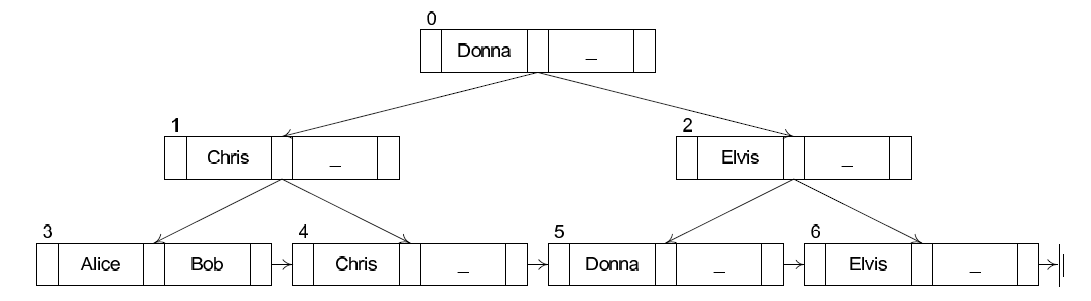
\includegraphics[scale=0.4]{img/btree.png}
\end{center}
\begin{center}
    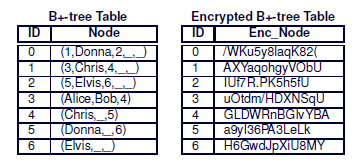
\includegraphics[scale=0.6]{img/tabtree.png}
\end{center}
Proviamo a fare una query su questo schema: 
\begin{minted}{sql}
    SELECT * FROM Accounts WHERE Customer = "Bob"
\end{minted}
Che viene interpretata ed eseguita così:
\begin{center}
    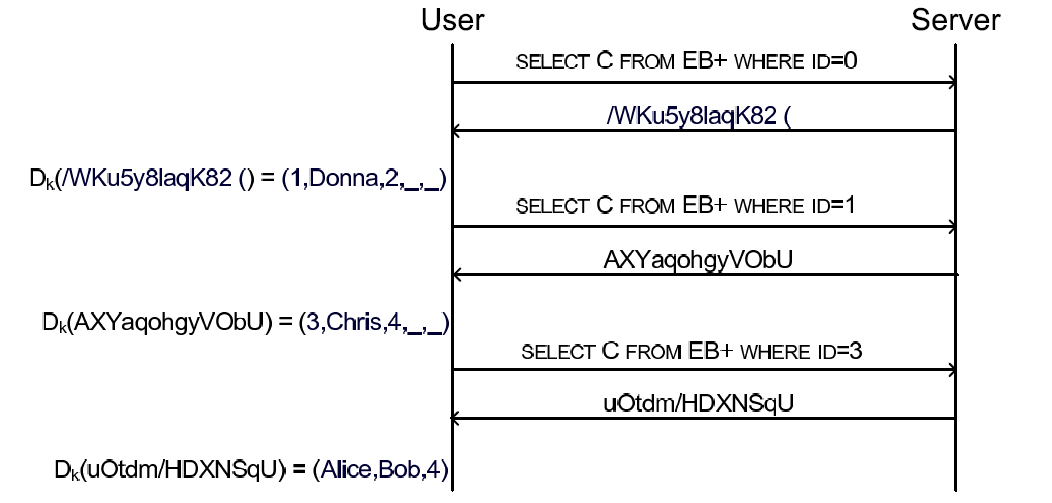
\includegraphics[scale=0.4]{img/treeinter.png}
\end{center}

\subsection{Searchable encryption}
\subsubsection{Order preserving}
\begin{itemize}
    \item \textbf{Order Preserving Encryption Schema (OPES)} prende in input una distribuzione target di valori di indici e applica una trasformazione che tiene conto dell' ordine in modo che i risultanti valori di indici seguano la distribuzione target. Vantaggi: la comparazione può essere effettuata direttamente sui dati criptati e la valutazione di query non produce risultati spuri. Svantaggi: è vulnerabile ad attacchi di inferenza.
    \item \textbf{Order Preserving Encryption with Splitting and Scaling (OPESS)} lo schema crea valori di indici tali che la loro distribuzione di frequenza sia piatta.
\end{itemize}
\subsubsection{Fully Homomorphic Encryption}
Questo metodo:
\begin{itemize}
    \item ci permette di eseguire specifiche computazioni sui dati criptati
    \item la decriptazione del risultato della computazione restituisce il risultato delle operazioni eseguite sui dati con il testo in chiaro.
\end{itemize}
Recenti avanzamenti hanno prodotto un functional-encryption schema che tiene insieme diversi schemi esistenti (homomorphic, garbled circuit ...), ma continua ad essere computazionalmente complesso per essere applicato ad un effettivo DBMS

\subsection{Inference Exposure}
Ci sono due conflitti di requisiti nell'indicizzazione dei dati:
\begin{itemize}
    \item gli indici devono fornire un meccanismo efficace di esecuzione delle query
    \item gli indici non dovrebbero permettere attacchi di inferenza o linking
\end{itemize}
È importante quindi misurare quantitativamente il livello di esposizione dovuto alla pubblicazione degli indici:\\
\begin{center}
    \( \epsilon\) = Coefficiente di Esposizione \\
\end{center}
La computazione del coefficiente di esposizione dipende sostanzialmente da due fattori:
\begin{itemize}
    \item il metodo di indicizzazione applicato:
    \begin{itemize}
        \item criptazione diretta
        \item hashing
    \end{itemize}
    \item la conoscenza che un intuso potrebbe avere a priori:
    \begin{itemize}
        \item \textbf{Freq + \(DB^k\)}: la distribuzione di frequenza dei valori in chiaro nel database originale (Freq), il database criptato (\(DB^k\))
        \item \textbf{DB + \(DB^k\)}: il database in chiaro (DB) e il database criptato \(DB^k\)
    \end{itemize}
\end{itemize}
Le inferenze a cui possiamo essere soggetti sono:\\
\textbf{Freq + \(DB^k\)}:
\begin{itemize}
    \item plaintext content: si può determinare l'esistenza di una certa tupla (o associazione di valori) nel db originale
    \item indexing function: si può determinare la corrispondenza tra indici e valori in chiaro
\end{itemize}
\textbf{DB + \(DB^k\)}:
\begin{itemize}
    \item indexing function: si può determinare la corrispondenza tra indici e valori in chiaro 
\end{itemize}
Andremo ad affrontare delle tecniche per calcolare il coefficiente di esposizione:
\begin{table}[h!]
\centering
 \begin{tabular}{| c || c| c |} 
 \hline
  & Direct Encryption & Hashing \\ [0.5ex] 
 \hline\hline
 Freq + \(DB^k\) & Quotient Table & Multiple subset sum problem \\ 
 \hline
 DB + \(DB^k\) & RCV graph & RCV line graph \\ [1ex] 
 \hline
 \end{tabular}
\end{table}

\subsubsection{Quotient table}
Vediamo un esempio di Freq + \(DB^k\): date queste conoscenze pregresse
\begin{center}
    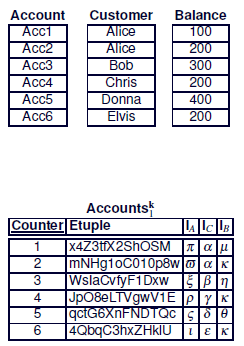
\includegraphics[scale=0.6]{img/freqdbk.png}
\end{center}
Le inferenze che possiamo fare sono:
\begin{itemize}
    \item \(I_A\) = Account 
    \item \(I_C\) = Customer 
    \item \(I_B\) = Balance
    \item \(\kappa \) = 200 (indexing inference)
    \item \( \alpha \) = Alice (indexing inference)
    \item \(<Alice,200>\) è nella tabella (association inference)
    \item Alice è associata anche con un valore diverso da 200 (100,300,400, tutti equiprobabili)
\end{itemize}
Cosa può espormi? Il fatto di essere particolare (Alice è l'unica che appare due volte)\\
Cosa può proteggermi? Il fatto che tutti gli altri siano come me.\\
La corrispondenza tra un indice e il valore in chiaro può essere determinata quindi dall'occorrenza dell'indice o del valore. La protezione più basica è quella di avere valori con lo stesso numero di occorrenza.\\
La valutazione dell'esposizione dell'indice è basata su una relazione di equivalenza dove indice/valore in chiaro con lo stesso numero di occorrenza appartengono alla stessa classe: l'esposizione dei valori nelle classe di equivalenza C è \( \frac{1}{|C|}\)
\begin{center}
    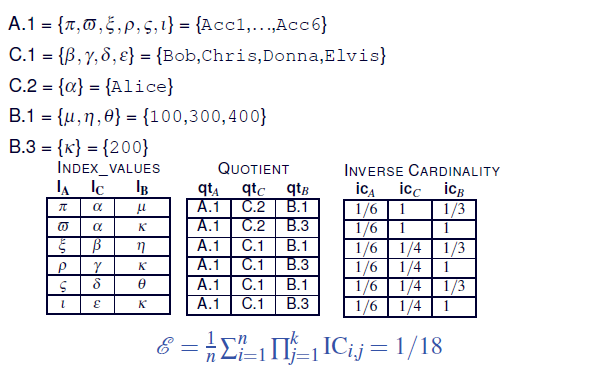
\includegraphics[scale=0.6]{img/quottable.png}
\end{center}
Come possiamo vedere dall'immagine abbiamo diverse sigle i cui nomi sono facilmente riconducibili all'attributo e alla sua occorrenza (A.1 attributo A che compare solo una volta, C.2 attributo C che compare due volte ecc...).\\
Il procedimento è il seguente:
\begin{enumerate}
    \item creo la tabella con i valori degli indici
    \item mappo la tabella degli indici in una nuova tabella di quozienti
    \item applicando la formula \( \frac{1}{|C|}\) ad ogni cella ottengo l'ultima tabella che rappresenta l'inverso della cardinalità. Da questa possiamo essere in grado di capire quali valori sono esposti e quali no, ad esempio i valori che hanno cardinalità inversa ad 1 sono esposti, mentre con  \( \frac{1}{|4|}\) ho il 25\% di possibilità di avere quel valore.
\end{enumerate}
L'ultima formula invece rappresenta l'esposizione totale della tabella:
\begin{itemize}
    \item 1..n sono le righe della tabella
    \item 1..k sono le colonne
    \item il calcolo è la somma dei prodotti dei valori di ogni riga
\end{itemize}

\subsubsection{RCV Graph}
L'obiettivo è quello di proteggere il mapping tra indici e valori in chiaro.\\
Il modello è rappresentato da un grafo colorato indiretto (non c'è verso negli archi) di tipo RCV (riga, colonna, valore) dove:
\begin{itemize}
    \item c'è un vertice di colore "colonna" per ogni attributo
    \item c'è un vertice di colore "riga" per ogni tupla
    \item c'è un vertice per ogni valore distinto in una colonna
    \item un arco connette ogni valore alla colonna e alla riga nella quale compare
\end{itemize}
RCV sui valori in chiaro è identico a quello sugli indici. \\
Il livello di esposizione può essere misurato valutando l'automorfismo del grafo. \\
Non è sufficiente contare il numero di automorfismi del grafo, infatti, se ci sono K automorfismi e in k di questi l'etichetta assegnata a v è la stessa, c'è una probabilita di \(\frac{k}{K}\) di identificare il valore.\\
Vediamo un esempio:
\begin{center}
    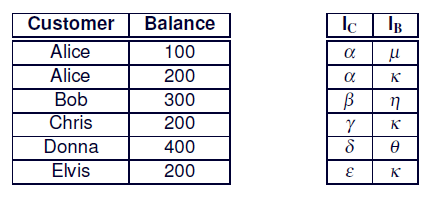
\includegraphics[scale=0.6]{img/dbdbk.png}
\end{center}
che viene rappresentata come:
\begin{center}
    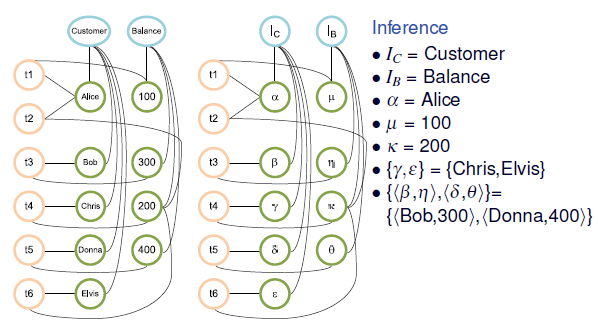
\includegraphics[scale=0.6]{img/expdbdbk.png}
\end{center}
L’insieme degli automorfismi forma un gruppo che è definito da una equitable partition, cioè la partizione dei nodi che si possono scambiare tra di loro (un nodo vale l’altro). Ogni sottoinsieme in una partizione è insieme con i nodi che si possono scambiare.\\
A questo punto posso utilizzare un algoritmo Nauty per derivare qualche partizione. Anche in questo caso la probabilità di individuare un elemento della partizione è \( \frac{1}{|C|}\).\\
Rifacendoci all'esempio di prima:\\
Equitable partition: \(\{(\alpha),(\beta,\delta),(\gamma, \epsilon),(\mu), (n,\theta),(\kappa)\}\) \\
Ho 9 elementi totali e 6 di confusione, quindi il mio coefficiente di esposizione è:
\(\Epsilon = \frac{6}{9} = \frac{2}{3} \)

\subsection{Bloom filter}
Il bloom filter è alla base della costruzione di alcune delle tecniche di indexing. È un metodo efficiente per codificare set membership (un dizionario su una struttura molto piccola). Gli elementi che lo definscono sono:
\begin{itemize}
    \item insieme di n elementi dove n è un numero molto alto
    \item vettore di l bits dove l è un numero piccolo (mi serve per mappare gli elementi)
    \item h funzioni di hash indipendenti \(H_i : \{0,1\}^* \rightarrow [1,l]\)
\end{itemize}
Per inserire un elemento x setto ad uno i bit alle posizioni degli indici \(H_1(x), H_2(x)..., H_h(x)\)\\
Per cercare un elemento x calcolo \(H_1(x), H_2(x)..., H_h(x)\) e controllo quale di quei valori sono settati nei bit del vettore.
\begin{center}
    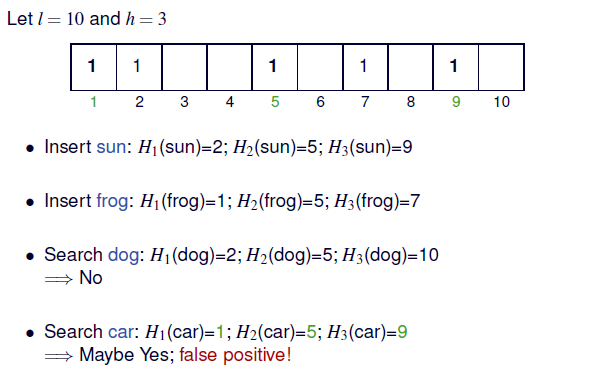
\includegraphics[scale=0.6]{img/bloomfliter.png}
\end{center}
Bloom filter con una sola funzione di hashing equivale all'hashing ordinario: occupano poco spazio (space efficient), ma gli elementi non possono essere rimossi.\\
Contiene falsi positivi (come abbiamo visto nell'esempio): nella teoria sono inaccettabili, ma nelle applicazioni pratiche è il prezzo da pagare per ottenere la space efficiency.

\subsection{Integrità dei Dati}
L'integrità dei dati si focalizza principalmente su due aspetti:
\begin{itemize}
    \item \textbf{integrità in storage}: i dati devono essere protetti da modifiche (le modifiche non autorizzare devono essere tracciate)
    \item \textbf{integrità nel calcolo delle query}: i risultati delle query devono essere corretti e completi (dobbiamo tracciare anche errori e mancamenti da parti del server nel calcolo di query)
\end{itemize}
Per garantire l'integrità dei dati in storage possiamo optare per le firme digitali che vengono calcolate solitamente a livello di tuple:
\begin{itemize}
    \item le firme di tabelle e attributi possono essere verificate solo dopo il download della tabella/colonna
    \item firmare a livello di cella causa un alto tasso di verifiche
\end{itemize}
Il costo della verifica crescwe linearmente con il numero di tuple nel risultato della query: le firme di un insieme di tuple possono essere combinate per generare firme aggregate

\subsection{Selective Encryption and Over-Encryption}
Siamo sempre nella situazione in cui uso un ente terzo per memorizzare i dati e voglio permetteer ad altri di accedere ai dati. Voglio avere la possibilità di eseguire query senza dare al server l' accesso ai dati in chiaro. Come si può fare? Faccio query direttamente sul criptato (crittografia diretta o omomorfica) oppure sfrutto gli indici, che però mi danno meno protezione.\\\\
Un'altra caratteristica che potrei volere è quella di differenziare gli utenti e con loro anche le viste nei dati pubblicati. Questo vorrebbe dire potenziare le policy di controllo di accesso che richiedono al data owner di mediare le richieste di accesso (soluzione impraticabile se non inapplicabile) oppure rafforzare le autorizzazioni che non dovrebbero essere delegate al provider (il data owner dovrebbe rimanere in pieno controllo dei suoi dati).\\
Abbiamo due tipi di approcci:
\begin{itemize}
    \item \textbf{Attribute-based encrypton (ABE)}: permette le derivazioni di una chiave solo da parte di utenti che possiedono certi attributi (basato su crittografia asimmetrica)
    \begin{center}
        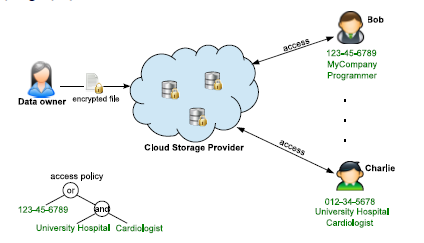
\includegraphics[scale=0.6]{img/abe.png}
    \end{center}
    
    \item \textbf{Selective encryption}: le policy di autorizzazione definite dal data owner vengono tradotte in policy di criptazione equivalenti 
    \begin{center}
        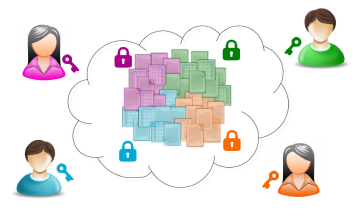
\includegraphics[scale=0.6]{img/selenc.png}
    \end{center}
\end{itemize}
Le idee che stanno alla base sono: 
\begin{itemize}
    \item i dati devono fare da soli il controllo sugli accessi
    \item dobbiamo usare chiavi differenti per criptare i dati
    \item l'autorizzazione per accedere a una risorsa viene tradottta in conoscenza delle chiavi con le quali le risorse sono criptate
    \item ad ogni utente vengono comunicate solo le chiavi necessarie a decriptare i dati e le risorse a cui può avere accesso.
\end{itemize}
\begin{center}
    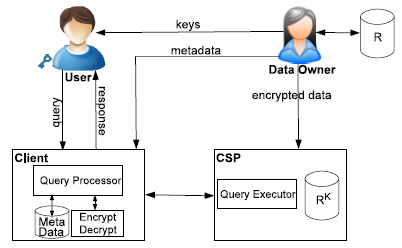
\includegraphics[scale=0.6]{img/selencscen.png}
\end{center}
Il data owner definisce una policy di controllo di accesso discrezionale per regolare l'accesso alle risorse. \\
Una policy di autorizzazione A è un set di permessi nella forma \(<user, resource>\) e può essere rappresentata come:
\begin{itemize}
    \item una matrice di accesso
    \item un grafo diretto che ha un vertice per ogni utente u e ogni risorsa r, e archi da u a r per ogni permesso \(<u, r>\)
\end{itemize}
Diverse ACLs implicano anche diverse chiavi di criptazione
\begin{center}
    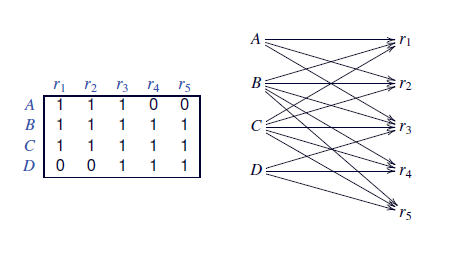
\includegraphics[scale=0.6]{img/authpolicy.png}
\end{center}
Come abbiamo detto in precedenza ogni policy di autorizzazione viene tradotta in un'equivalente policy di criptazione.\\
Abbiamo diverse possibili soluzioni:
\begin{itemize}
    \item cripto ogni risorsa con una chiave diversa e consegno ad ogni utente le chiavi delle risorse a cui può accedere (richiede agli utenti di gestire tante chiavi quanti i numeri di risorse a cui sono autorizzati ad accedere)
    \item usare un metodo di derivazione delle chiavi per permettere agli utenti di derivare dalle chiavi tutte le altre a cui possono avere accesso (posso quindi dare una sola chiave ad ogni utente)
\end{itemize}
Abbiamo citato il metodo di derivazione delle chiavi, andiamo ad approfondirlo.\\
Questo è basato su una gerarchia di derivazione delle chiavi (\(K, \preceq\)) dove K è l'insieme di chiavi nel sistema, e \(\preceq\) è l'ordine parziale definito su K \\
La conoscenza della chiave del vertice \(v_1\) e di una parte dell'informazione disponibile pubblicamente permette il calcolo della chiave di un livello inferiore \(v_2\) tale che \(v_2 \preceq v_1 \).\\
(\(K, \preceq\)) può essere rappresentato tramite un grafo dove ogni nodo rappresenta una chiave x nell'insieme K ed esiste l'arco da x a y sse \(y \preceq x \) \\
In base alla funzione di ordine parziale definita su K, la gerarchia di derivazione delle chiavi può essere:
\begin{itemize}
    \item una catena
    \item un albero
    \item un DAG
\end{itemize}
Le chiavi vengono arbitrariamente assegnate ai vertici. Viene associata anche un'etichetta l ad ogni chiave k. Una parte dell'informazione pubblica \(t_{i,j}\) chiamata \textbf{token} è associata ad ogni arco nella gerarchia.\\
Dato un arco (\(k_i, k_j\)), il token \(t_{i,j}\) è calcolato come \(k_j \oplus h(k_i, l_j)\) dove:
\begin{itemize}
    \item \(\oplus\) è l'operatore xor n-ario
    \item h è una funzione di hash sicura
\end{itemize}
I vantaggi principali di utilizzare i tokens:
\begin{itemize}
    \item sono pubblici e permettono agli utenti di derivare chiavi di criptazione multiple, preoccupandosi di gestirne solo una
    \item possono essere salvati in un server remoto (come i dati criptati) così che ogni utente possa accederci
\end{itemize}
Le relazioni tra le chiavi e i token possono essere rappresentati tramite un grafo \textbf{key and token} dove abbiamo:
\begin{itemize}
    \item un vertice \(<k,l>\), dove \(k \in K\) è una chiave e \(l \in L\) è la corrispondente etichetta
    \item un arco da un vertice \(<k_i,l_i>\) al vertice \(<k_j,l_j>\) se esiste un token \(t_{i,j} \in T\) che permette la derivazione di \(k_j\) a partire da \(k_i\)
\end{itemize}
\begin{center}
    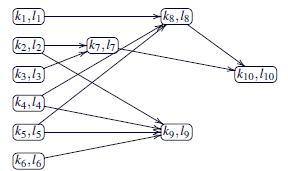
\includegraphics[scale=0.7]{img/ktgrafo.png}
\end{center}
Nell'esempio riportato sopra conoscendo \(k_1\) posso derivare \(k_8\) e \(k_10\) \\\\
Come abbiamo detto in precedenza dobbiamo tradurre le policy di autorizzazione in policy di criptazione. Assunzioni iniziali:
\begin{itemize}
    \item ad ogni utente deve essere rilasciata una sola chiave
    \item ogni risorsa è criptata una sola volta (con una sola chiave)
\end{itemize}
Abbiamo quindi una funzione \(\phi : U \cup R \righarrow L \) che descrive le associazioni tra utenti e (l'etichetta della loro) chiave e l'associazione tra risorse e(l'etichetta della) chiave usata per criptarla.\\
Definiamo formalmente policy di criptazione:\\
una policy di criptazione sugli utenti U e risorse R, denotata con \(\epsilon\), è una sestupla \(<U,R,K,L,\phi,t>\) dove:
\begin{itemize}
    \item K è l'insieme delle chiavi definite nel sistema e L è l'insieme di etichette corrispondenti
    \item \(\phi\) è un assegnamento di una chiave e uno schema di criptazione
    \item T è un insieme di token definito su K e L
\end{itemize}
Anche questo tipo di policy può essere rappresentata attraverso un grafo estendendo quello visto precedentemente per includere:
\begin{itemize}
    \item un vertice per ogni utente e ogni risorsa
    \item un arco che collega ogni utente u al vertice \(<k,l>\) tali che \(\phi(u) = l \)
    \item un arco che collega ogni vertice \(<k,l>\) ad ogni vertice delle risorse tali che \(\phi(r) = l \)
\end{itemize}
\begin{center}
    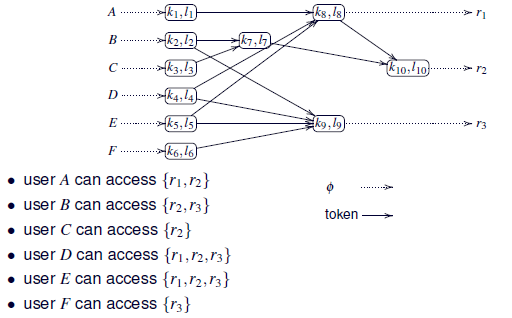
\includegraphics[scale=0.7]{img/epolicy.png}
\end{center}
L'obiettivo della traduzione è quello di tradurre una policy di autorizzazione A in una policy di criptazione equivalente \(\epsilon\).\\
A ed \(\epsilon\) sono equivalenti se garantiscono gli stessi accessi, senza garantire di più o di meno.\\
Questa traduzione può essere eseguita in due modi:
\begin{itemize}
    \item approccio naive: ogni utente è associato ad una chiave differente, ogni risorsa è associata con una chiave diversa, un token \(t_{u,r}\) è generata e pubblicata per ogni permesso \(<u,r>\), ma produrre e gestire un token per ogni permesso può essere infattibile praticamente
    \item creare ACL: creo gruppi di utenti con gli stessi privilegi e cripto risorse con chiave data a tutto il gruppo
\end{itemize}
È possibile creare un grafo di policy di criptazioni sfruttando la gerarchia tra insiemi di utenti indotti dalla relazione di ordine parziale. \\
Se il sistema ha un grande numero di utenti la policy di criptazione ha un grande numero di token e chiavi (\(2^{|U|-1}\))
\begin{center}
    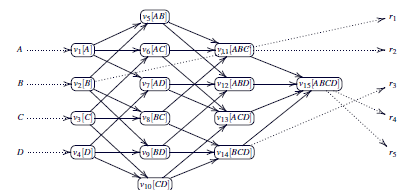
\includegraphics[scale=0.7]{img/transpolicy.png}
\end{center}
Possiamo notare come i gruppi di utenti che non corrispondo a nessun ACL non abbiano nessuna chiave. L'obiettivo è quindi quello di calcolare la policy di criptazione minima che minimizza il numero di token che deve essere mantenuto dal server. Le possibili soluzioni sono algoritmi euristici basati su osservazioni:
\begin{itemize}
    \item solo i vertici associati a gruppi di utenti che corrispondo a delle ACL devono essere associate ad una chiave
    \item il grafo delle policy di criptazione può includere solo i verci che servono per imporre una certa policy di autorizzazione, connettendoli per garantire una corretta derivazione di chiavi
    \item altri vertici possono essere inclusi se sono utili per ridurre la dimensione del catalogo
\end{itemize}
Per costruire un grafo di chiavi e token abbiamo 3 fasi:
\begin{enumerate}
    \item \textbf{Inizializzazione}: creo un vertice/chiave per ogni utente e per ogni ACL non singleton
    \item \textbf{Copertura}: per ogni vertice v corrispondente a un ACL non singleton troviamo una copertura senza ridondanza (deve coprire l'insieme)
    \item \textbf{Fattorizzazione}: fattorizzare gli antenati comuni
\end{enumerate}
\begin{center}
    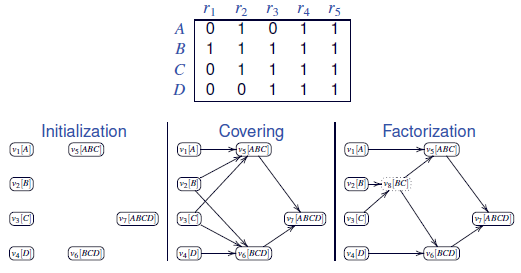
\includegraphics[scale=0.7]{img/keytoken.png}
\end{center}
A questo punto la mia policy di criptazione è decisa.
Dal token graph (l'ultimo a destra) posso dare a ciascun utente la sua chiave e criptare ogni risorsa con la sua chiave, creando così la tabella dei token:
\begin{center}
    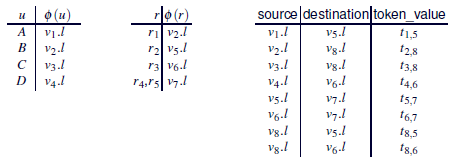
\includegraphics[scale=0.7]{img/tokentab.png}
\end{center}
Quando proprietari diversi hanno bisogno di condividere i loro dati, l'uso di una chiave permette a due proprietari di condividere una chiave segreta per seguenti usi crittografici.\\
Quando si autorizzano cambiamenti dinamici, il proprietario dei dati deve:
\begin{itemize}
    \item scaricare le risorse dal server
    \item creare una nuova chiave per le risorse
    \item decriptare la risorsa con la vecchia chiave
    \item criptare le risorse con la nuova chiave
    \item caricare le risorse sul server e comunicare i cambiamenti
\end{itemize}
Possiamo notare come questo procedimento sia davvero inefficiente e per questo subentra \textbf{over-encryption}.\\
Il funzionamento è semplice: le risorse sono criptate due volte:
\begin{itemize}
    \item dal proprietario con una chiave condivisa con gli utenti e sconosciuta al server (Base Encryption Layer - BEL level)
    \item dal server, con una chiave condivisa con gli utente autorizzati (Surface Encryption Layer - SEL level)
\end{itemize}
Per accedere ad una risorsa un utente deve sapere entrambe le chiavi BEL e SEL.\\
Garantire e revocare le operazioni può richiedere l'aggiunta di nuovi token a BEL level e l'aggiornamento del SEL level in conseguenza alle operazioni eseguite.\\
A livello BEL possiamo distinguere due chiavi, una di accesso \(k_a\) e una di derivazione (k):
\begin{itemize}
    \item ogni nodo in Bel è associato con una coppia di chiavi (k,\(k_a\)) dove \(k_a = h(k)\) dove h è una funzione di hash, e una coppia di (\(l,l_a\))
    \item la chiave k con etichetta l è usata per scopi di derivazione
    \item la chiave \(k_a\) con etichetta \(l_a\) è usata per criptare le risorse associate al nodo
    \item questa distinzione separa i due ruoli associati alle chiavi: abilita la derivazione della chiave e abilita l'accesso alla risorsa
\end{itemize}
Il livello SEL è caratterizzato da una policy di criptazione definita come illustrato precedentemente. Esistono due tipi di SEL:
\begin{itemize}
    \item \textbf{Full\_SEL}: parte da una SEL identica alla BEL e tiene SEL sempre aggiornata per rappresentare la policy corrente (tutte le risorse sono criptate)
    \item \textbf{Delta\_SEL}: parte da una SEL vuota e aggiunge elementi man mano che la policy si evolve, in modo che la coppia BEL-SEL rappresenti la policy (server cripta solo quando serve coprire qualcosa, se non cambia la politica non ha senso cambiare ancora)
\end{itemize}
Vediamo un esempio:
\begin{center}
    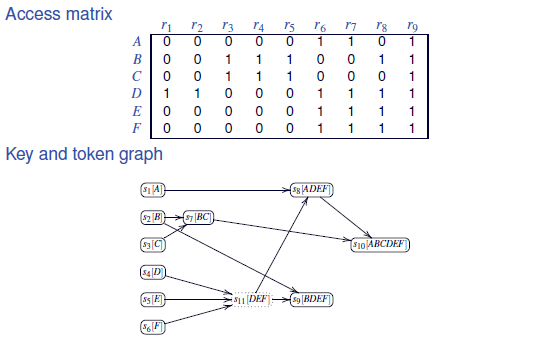
\includegraphics[scale=0.7]{img/belsel1.png}
\end{center}
\begin{center}
    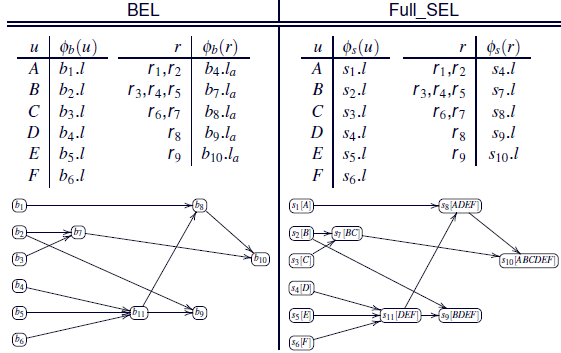
\includegraphics[scale=0.7]{img/belsel2.png}
\end{center}
\begin{center}
    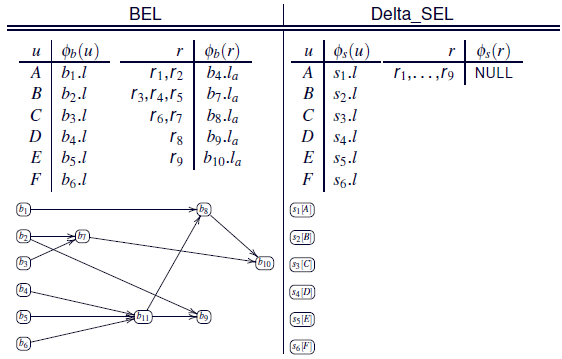
\includegraphics[scale=0.7]{img/belsel3.png}
\end{center}
Le evoluzioni di BEL e SEL sono gestite da:
\begin{itemize}
    \item procedure over-encrypt (lato SEL) che regolano il processo di aggiornamento attraverso l'over-encrypting delle risorse a livello SEL. Il server riceve una richiesta per sovrascrivere una risorsa per un gruppo di utenti (cioè per sovrascrivere una risorsa così da renderla disponibile solo per quel gruppo di utenti). Se la risorsa è già sovra criptata allora il server la apre e, se non esiste una chiave che corrisponde a un insieme di utenti, il server crea la chiave. Infine il server cripta le risorse con la nuova chiave.
    \item garantisce e revoca le procedure che servono per garantire e revocare privilegi. 
    \begin{itemize}
        \item Nel caso del grant (lato BEL): voglio garantire ad un utente l’accesso a una risorsa che è criptata con una certa chiave. Quindi voglio aggiungere l’utente all’ACL della risorsa. Se l’utente non riesce a derivare la chiave, aggiungo un token per derivare quella chiave. Se ad esempio questo nuovo utente non può accedere alle risorse della chiave che gli è stata data, allora il server crea delle partizioni (in base all’ACL) e fa over encryption. A questo punto come faccio a fare in modo che il server sappia che il nuovo utente può accedere alla risorsa? Il server fa over encryption.
        \item Nel caso del revoke (lato BEL): l’utente può accedere alla risorsa; l’obiettivo è togliergli l’accesso. Lato proprietario si aggiorna l’ACL. Il server deve restringere l'accesso alla risorsa facendo over encryption.
    \end{itemize}
\end{itemize}
Le policy di criptazione BEL e SEL sono equivalenti alle policy di autorizzazione dichiarate durante la fase di inizializzazione. Le procedure viste poco fa preservano l'equivalenza, la funzione di derivazione delle chiavi che è stata adottata è sicura, tutte le funzioni di criptazione e i token sono robusti e non possono essere rotte. Ogni utente può maneggiare correttamente le sue chiavi senza la possibilità di poter rubare quelle di un altro utente.\\
Nonostante ciò si è vulnerabili agli attacchi di collusione: combinando le conoscenze due o più entità riescono a conoscere cose a cui nessuo di loro avrebbe accesso. Le collusioni possono essere tra utenti e col server. L'attacco dipende dalle diverse viste che gli attaccanti hanno nei confronti di una certa risorsa r. \\
Abbiamo quattro possibili scenari:
\begin{itemize}
    \item open: l'utente conosce le chiavi del BEL e del SEL
    \item locked: l'utente non conosce nessuna chiave
    \item sel\_locked: l'utente conosce solo la chiave del BEL
    \item bel\_locked: l'utente conosce solo la chiave del SEL
\end{itemize}
Il server ha sempre un tipo di vista bel\_locked.
\begin{center}
    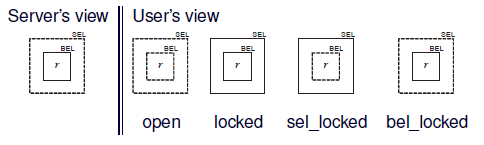
\includegraphics[scale=0.7]{img/selbellock.png}
\end{center}
Ogni livello è rappresentato come una ringhiera: discontinuo se la chiave è conosciuta, continuo se la chiave è sconosciuta.\\
Mi proeccupo delle collisioni in sel\_locked, cioè quando l'utente e il server sanno qualcosa e mettono insieme.\\\\
Consideriamo una risorsa r e la storia della sua acl(r). Gli utenti presenti in questa storia possono essere classificati in quattro categorie:
\begin{center}
    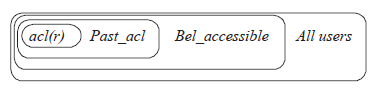
\includegraphics[scale=0.6]{img/classuser.png}
\end{center}
C'è rischio di collusione per r sse ci sono utenti in Bel\_Accessible che non appartengono a Past\_acl (ha un accesso a cose a cui non ha mai avuto accesso).\\\\

Un utente può avere la vista sel\_locked su r se (chiedere la criptazione lato server) se:
\begin{itemize}
    \item utente autorizzato e lo sto revocando
    \item risorsa coinvolta in policy split: l'utente ha accesso ad r' (non a r), criptato a livello BEL con la stessa chiave di r. Quindi devo chiedere la criptazione lato SEL per evitare che l'utente acceda anche ad r avendo la sua chiave.
\end{itemize}
\begin{center}
    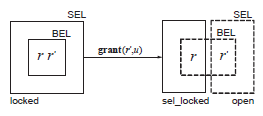
\includegraphics[scale=0.7]{img/seltrans.png}
\end{center}
Abbiamo la stessa cosa anche nel Delta\_SEL (sempre per un problema di policy split):
\begin{center}
    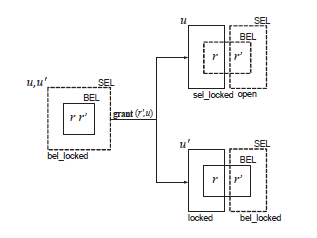
\includegraphics[scale=0.7]{img/deltatrans.png}
\end{center}
Quindi ricapitolando:
\begin{itemize}
    \item in Full\_SEL
    \begin{itemize}
        \item tra gli utenti non c'è problema, gli utenti non guadagnano mai nello scambio
        \item col server è possibile che ci siano collusioni, ma sono facilmente identificabili ed evitabili tramite re-criptazione
    \end{itemize}
    \item in Delta\_SEL ci sono problemi se lato utente al tempo 0 mi scarico tutto quello che viene messo fuori in un secondo momento posso usare la chiave che ho io per accedere alle risorse.
\end{itemize}

\subsection{Frammentazione e criptazione}
La criptazione rende la valutazione delle query e l'esecuzione delle applicazioni più costose o non sempre possibili.\\
Spesso la cosa più sensibile è l'associazione tra due valori di due attributi (più che i valori presi singolarmente) e per proteggere tale associazione si potrebbe romperla al posto che criptarla.\\
Abbiamo dei vincoli di confidenzialità che vengono specificati dall'utente e possono essere riferiti ai singoli attributi o alle associazioni. Per esempio dato R = (Name, DoB, Gender, Zip, Position, Salary, Email, Telephone)
\begin{itemize}
    \item \{Telephone\},\{Email\}: sono sensibili e non possono essere salvati in chiari
    \item \{Name, Salar\}, \{Name, Position\}, \{Name, DoB\}: gli attributi Salary, Position, DoB sono privati di un individuo e non possono essere salvati in chiaro con l'associazione col nome
    \item \{DoB, Gender, Zip, Salary\}, \{DoB, Gender, Zip, Position\}: gli attributi DoB, Gender, Zip potrebbero essere dei quasi identificatori
    \item \{Position, Salary\}, \{Salary, DoB\}: le regole di associazione tra Position e Salary e tra Salary e DoB dovrebbero essere protette da un attaccante 
\end{itemize}

\subsubsection{Server non comunicanti}
I vincoli di confidenzialità sono rinforzati dividendo le informazioni su due server indipendenti che non possono comunicare. Così facendo le associazioni sensibili sono protette distribuendo gli attributi tra i due server e la criptazione è applicata solo quando viene esplicitamente chiesto dai vincoli di confidenzialità o quando salvare un attributo in chiaro in uno dei due server potrebbe esporre almeno un'associazione sensibile.\\
Il vincoli di confidenzialità C definiti su una relazione R sono rafforzati dividendo R in \(<R_1, R_2, E>\) dove:
\begin{itemize}
    \item \(R_1\) e \(R_2\) includono un tuple ID univoco necessario per garantire una divisione senza perdite
    \item \(R_1 \cup \R_2 = R\)
    \item E è il set di attributi criptati e \( E \subseteq R_1\), \( E \subseteq R_2\)
    \item per ogni \(c \in C\), \(c \nsubseteq (R_1 - E)\) e \(c \nsubseteq (R_2 - E)\) 
\end{itemize}
Per ricostruire i frammenti devo avere in comune qualcosa che è chiave, ad esempio un tuple ID. Inoltre, nessuno dei due frammenti contiene in chiaro attributi che fanno tutti parte di un vincolo di confidenzialità. Un vincolo di confidenzialità non è contenuto nella sua globalità in nessuno dei frammenti in chiaro.
\begin{center}
    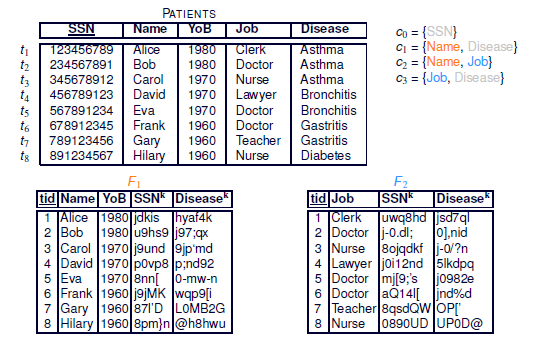
\includegraphics[scale=0.7]{img/noncommserv.png}
\end{center}
\paragraph{Come si eseguono le query?}\\
A livello logico rimpiazzo R con la join tra \(R_1 \bowtie R_2\).
Quindi faccio la query sul join, sfruttando il più possibile i server. Posso eseguire la query in due modi: 
\begin{itemize}
    \item eseguo le due query in parallelo, faccio il join e ho il risultato \(\rightarrow\) se i server conoscono la query i miei dati sono esposti
    \item faccio la query da una parte e poi faccio un semi join con l’altra tabella sfruttando il tuple ID (esempio: estraggo le persone nate dopo il 2000, prendo il tuple ID di queste persone e utilizzo i tuple ID per andare a prendere i dati nell’altro frammento, così non devo scaricare tutti i dati) \(\rightarrow\) comunico al server quali tuple ID mi servono
\end{itemize}
\paragraph{Come faccio la frammentazione?}\\
Applichiamo un approccio brute force per ottimizzare il carico di lavoro W:
\begin{itemize}
    \item per ogni possibile decomposizione sicura di R:
    \begin{itemize}
        \item ottimizzo ogni query in W per la decomposizione
        \item stimo il costo totale per eseguire le query in W usando il piano di query ottimizzate
    \end{itemize}
    \item seleziono la decomposizione che ha il minor costo totale
\end{itemize}
Questo però è un approccio troppo costoso.\\
Usiamo quindi la matrice di affinità: attributi sulle righe e sulle colonne, la cella i,j mi dice quante volte gli attributi i e j compaiono insieme nelle query. La diagonale principale mi dice quanto costa criptare quell'attributo. Per ottimizzare andrò a criptare e frammentare in modo tale da pagare il minor costo possibile quando andrò a fare le query.\\
Formalmente vogliamo minimizzare:
\[\sum_{i,j: i \in (R_1 - E), j \in (R_2-E)} M_{i,j} + \sum_{i \in E}M_{i,i}\]
Questo problema è equivalente al problema di colorazione di un ipegrafo (un ipergrafo è una generalizzazione di un grafo dove gli archi possono collegare qualsiasi numero di vertici - ogni server ha un colore diverso) dove gli attributi sono vertici, la matrice di affinità mi dà il peso degli archi, la diagonale principale mi dà il peso dei vertici. I vincoli di confidenzialità C rappresentano un ipergrafo H(R,C) sugli stessi vertici.\\
Dobbiamo trovare la soluzione in modo che:
\begin{itemize}
    \item nessun arco sia monocromatico
    \item il peso dei vertici bicromatici sia minimizzato
    \item un vertice può essere cancellato pagando il peso dei vertici
\end{itemize}
Anche in base alla formula di prima abbiamo che:
\begin{itemize}
    \item il peso degli archi bicromatici è \(\sum_{i,j: i \in (R_1 - E), j \in (R_2-E)} M_{i,j} \)
    \item il peso della cancellazione di un vertice è \(\sum_{i \in E}M_{i,i}\)
\end{itemize}
L'obiettivo è sempre quello di minimizzare la somma vista in precedenza.\\
Cosa ho alla fine: due frammenti, qualcosa in chiaro e qualcosa criptato.\\
Problemi della tecnica che si basa su server non comunicanti: muro che c’è fra i due server, l’assunzione di avere questo muro è un po’debole nel mondo odierno.

\subsubsection{Frammenti non linkabili}
L'accoppiata frammentazione/criptazione è interessante e porta molti vantaggi ma assumere che ci siano due server non comunicanti:
\begin{itemize}
    \item è difficile da forzare nella realtà
    \item limita il numero delle associazioni che possono essere risolte frammentando i dati
\end{itemize}
Una frammentazione di R è un insieme di frammenti \( F = \{F_1,..., F_m\}\) dove \(F_i \subseteq R\) per \(i=1,...,m\)\\
Una frammentazione F di R rafforza correttamente un insieme di vincoli di confidenzialità C sse le seguenti condizioni sono verificat:
\begin{itemize}
    \item ogni singolo frammento soddisfa i vincoli
    \item i frammenti non hanno attributi in comune, altrimenti avrei la possibilità di fare linking
\end{itemize}
Ogni frammento F è mappato in un frammento fisico contenente:
\begin{itemize}
    \item gli attributi nel frammento in chiaro
    \item tutti gli altri attributi di R criptati (viene applicato salt ad ogni criptazione)
\end{itemize}
\begin{center}
    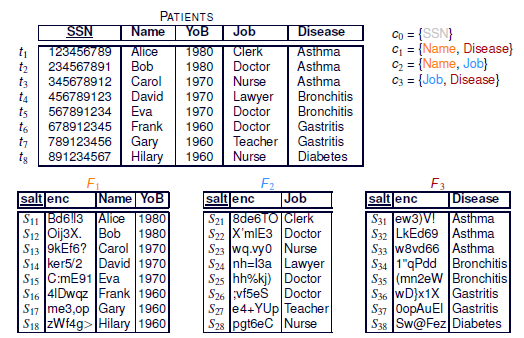
\includegraphics[scale=0.7]{img/nonlink.png}
\end{center}
\paragraph{Come si eseguono le query?}\\
Non mi serve più andare a recuperare tutti i frammenti, me ne basta uno. Se la query coinvolge un attributo criptato potrebbe essere necessaria un'altra query lato client.\\
Se volessi trovare le malattie dei pazienti nati dopo il 1980 farei una query sul frammento dove c'è la data di nascita così da avere meno tuple da decriptare per avere la malattia.

\paragraph{Come frammentiamo?}\\ Come frammentiamo e soprattutto rispetto a cosa frammentiamo? L'obiettivo che vogliamo ottenere è quello di avere una frammentazione che mi permette di eseguire query efficienti. Possiamo frammentare in base a tre criteri:
\begin{itemize}
    \item numero di frammenti
    \item affinità tra gli attributi
    \item query workload
\end{itemize}
Tutti i criteri devono rispettare il criterio di massima visibilità: solo gli attributi che appaiono in vincoli singleton (attributi sensibili) devono essere criptati, tutti gli altri attributi non sensibili devono avere almeno un frammento in cui siano in chiaro.\\
Quello che vogliamo fare è minimizzare la frammentazione. Per ridurre la complessità vogliamo determinare una frammentazione corretta ma col minor numero di frammenti.\\
Una frammentazione è minimale se tutte le frammentazioni che possono essere ottenute dalla frammentazione minimale unendo qualsiasi coppia di frammenti, viola almeno un vincolo.
\begin{center}
    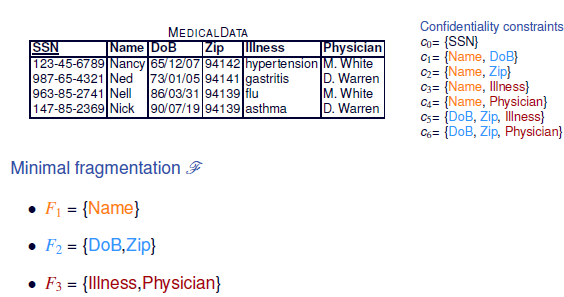
\includegraphics[scale=0.7]{img/fragment.png}
\end{center}
Unendo due dei frammenti si violerebbe almeno un vincolo.\\
Anche in questo caso ho una matrice di affinità. I frammenti vengono calcolati considerando gli attributi che più "vogliono" stare insieme (maximum affinity).\\
Per calcolare maximum affinity si può usare un'euristica che ad ogni passo prende la mossa migliore.\\
Vediamo un esempio:
\begin{center}
    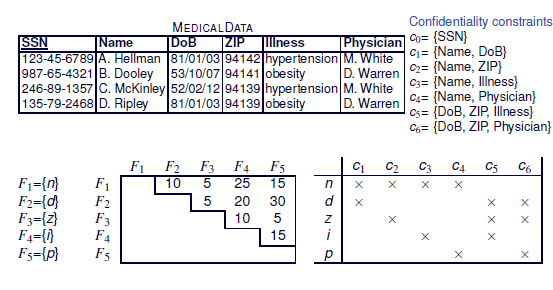
\includegraphics[scale=0.7]{img/maxaff1.png}
\end{center}
In quest'immagine possiamo vedere una tabella di medical data, dei vincoli di confidenzialità e delle frammentazioni di base. La matrice in basso a sinistra rappresenta la matrice di affinità ed è scritta per metà poichè la metà sotto sarebbe uguale a quella sopra e la diagonale, non essendoci nulla di criptato, è cancellata. La matrice in basso a destra rappresenta gli attributi e i vari vincoli a cui sono legati.
\begin{center}
    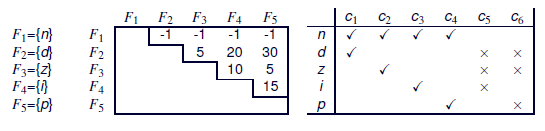
\includegraphics[scale=0.7]{img/maxaff2.png}
\end{center}
In questa foto possiamo vedere come tutta la prima riga della matrice dei frammenti sia stata messa a -1. Questo è avvenuto perchè l'attributo name (contenuto nel frammento F1), per i vincoli di confidenzialità, non può stare con nessun altro attributo (altrimenti violerebbe i vincoli). Mettendo a -1 il valore non andremo a considerarli successivamente.\\
Facendo la mossa localmente migliore (in un algoritmo con approccio greedy) so che otterrò un risultato che è globalmente migliore. Quindi in questo caso la mossa migliore è unire F2 ed F5 (visto che il loro incrocio ha valore 30) e facendo questo vuol dire che F5 sparisce e dobbiamo regolare le affinità di F2.\\
Le nuove affinità si calcolano come seguono:
\begin{itemize}
    \item F3 voleva stare 5 con F5, quindi visto che ora F5 sta con F2, aggiungiamo 5 all'incrocio F2/F3
    \item F4 voleva stare 15 con F5, quindi visto che F5 sta con F2, aggiungiamo 15 all'incrocio F2/F4
\end{itemize}
\begin{center}
    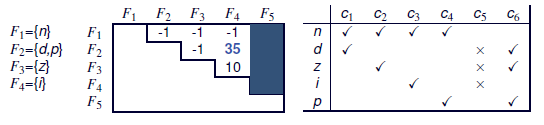
\includegraphics[scale=0.7]{img/maxaff3.png}
\end{center}
Quello che succede è che dovrei avere l'incrocio F2 (DoB e Physician) F3 (ZIP) che vale 10, ma in realtà vale -1, perchè il vincolo c6 ci dice che questi tre attributi non possono stare insieme.
\begin{center}
    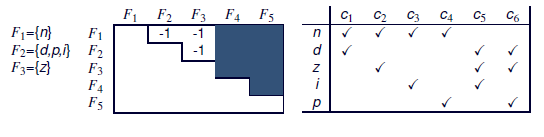
\includegraphics[scale=0.7]{img/maxaff4.png}
\end{center}
Eseguendo una nuova iterazione otteniamo la situazione riportata sopra dove non possiamo più eseguire mosse avendo solo valori negativi.\\
L'affinità massima di frammentazione F vale 65.
È la soluzione ottima poichè mettendo insieme due frammenti si violerebbe almeno un vincolo.\\\\


\subsection{Frammentazione}
\subsubsection{Keep a few}
L'idea che sta alla base è che:
\begin{itemize}
    \item  la criptazione rende il processo di esecuzione delle query più costoso e non sempre possibie
    \item la criptazione porta a dover gestire un numero grande di chiavi
\end{itemize}
Perchè non eliminare del tutto la criptazione?\\
Il problema è capire quanto posso caricare su server esterni, l'obiettivo infatti è tenere il meno possibile.\\
Devo determinare una frammentazione a due dove uno sono io (l'owner) e uno è il server.\\
Dati \(R(A_1,...,A_n)\) uno schema relazionale e \(C=\{c_1,...,c_m\}\) vincoli di confidenzialità su R, vogliamo determionare una frammentazione \(F=<F_O,F_S>\) dov:
\begin{itemize}
    \item \(F_O \cup F_S = R\) (\textbf{completezza})
    \item \(\forall c \in C, c\nsubseteq F_S\) (\textbf{confidenzialità})
    \item \(F_O \cap F_S = \emptyset \) (\textbf{non ridondanza})
\end{itemize}
A livello fisico \(F_O\) e \(F_S\) hanno un attributo comune (tid) per permettere l'esecuzione di join senza perdite di dati.
\begin{center}
    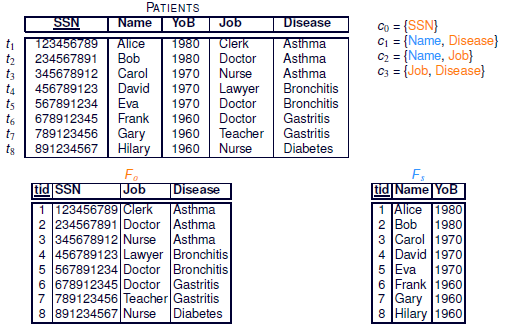
\includegraphics[scale=0.7]{img/keepafew.png}
\end{center}
\subsection{Valutazione di Query}
Una query può avere dentro delle condizioni che possono coinvolgere attributi miei (\(C_O\)), del server (\(C_S\)) o di entrambi (\(C_SO\)). Devo tradurre la mia query in query equivalenti che lavorano lato mio, lato server e combinato.\\
Usando come esempio i frammenti precedenti proviamo a capire la valutazione della query:
\begin{minted}{sql}
    SELECT SSN,YoB
    FROM Patients
    WHERE (Disease = "Bronchitis") AND (YoB = "1970") AND (Name = Job)
\end{minted}
Le condizioni dello WHERE sono divise in:
\begin{itemize}
    \item (\(C_O\)) = \{Disease = "Bronchitis"\}
    \item (\(C_S\)) = \{YoB = "1970"\}
    \item (\(C_SO\)) = \{Name = Job\}
\end{itemize}
Abbiamo diverse strategie da poter adottare:
\begin{itemize}
    \item Server-Client strategy 
    \begin{enumerate}
        \item il server valuta (\(C_S\)) e ritorna il risultato al client
        \item il client riceve il risultato ed esegue la join con il suo frammento
        \item il client valuta (\(C_SO\)) e (\(C_O\)) sul join
    \end{enumerate}
    \item Client-Server strategy
    \begin{enumerate}
        \item il client valuta (\(C_O\)) e manda al server la serie di tid
        \item il server fa la join col suo frammento ed esegue la sua query ritornando il risultato al client
        \item il client esegue la join del suo frammento con il risultato del server e valuta (\(C_SO\)) 
    \end{enumerate}
\end{itemize}
Quale delle due strategie è meglio?\\
Se il server conosce o può fare inferenza sulle query il modello Client-server perde informazioni: il server può fare inferenza sulle tuple che sono associate con i valori che soddisfano (\(C_O\)).\\
Se il server non conosce e non può fare inferenza sulle query: possiamo adottare qualsiasi strategia senza preoccuparci di violazioni di privacy (scegliendo magari quella più performante).\\
Il mio obiettivo è quello di minimizzare il carico di lavoro dell'owner.\\
La funzione peso w prende una coppia \(<F_O, F_S>\) come input e ritorna il carico di lavoro dell'owner.\\
Una frammentazione \(F = <F_O, F_S>\) è minimale sse:
\begin{enumerate}
    \item F è corretta (soddisfa completezza, confidenzialità e non ridondanza)
    \item non esiste F' tale che \(w(F') < w(F)\) e F' è corretta
\end{enumerate}
Possiamo adottare diverse tecniche per dividere gli attributi tra \(F_O\) e \(F_S\) che minimizzano:
\begin{itemize}
    \item storage: numero di attributi (Min-Attr) o dimensioni degli attributi (Min-Size)
    \item traffico/computazione: numero di query nelle quali è richiesto l'intervento dell'owner (Min-Query) o numero di condizioni all'interno delle query nelle quali l'owner deve essere coinvolto (Min-Cond)
\end{itemize}
Vediamole nel dettaglio:
\begin{itemize}
    \item Min-Attr: minimizzo il numero di attributi nel frammento dell'owner
    \item Min-Size: minimizzo la dimensione fisica del frammento dell'owner (somma del peso fisico degli attributi)
    \item Min-Query: minimizzo il numero di query che richiedono lavoro all'owner (somma delle frequenze delle query)
    \item Min-Cond: minimizzo il numero di condizioni che richiedono del lavoro all'owner
\end{itemize}
Abbiamo così espresso tutte le metriche con un peso, tra queste cambia la forma del peso.
A questo punto, dato il nostro problema e dato il nostro peso da minimizzare che ci verrà dato, dobbiamo trovare alcuni attributi da mettere in \(F_O\) e in \(F_S\) in modo da minimizzare il peso (uno dei quattro casi visti qui sopra).
Rappresentiamo tutti i criteri con un modello uniforme basato su:
\begin{itemize}
    \item insieme target: elementi rispetto ai quali è definito il problema di minimizzazione
    \item funzione peso: associa il peso a ogni elemento target
    \item peso dell'insieme di attributi: somma dei pesi dei target intersecati all'insieme
\end{itemize}
L'obiettivo è calcolare l'insieme di attributi con il minor peso, per farlo devo minimizzare la somma dei target che fanno parte dell'hitting set (uso un'euristica che mi assicura minimalità).\\
Questa euristica prende in input:
\begin{itemize}
    \item A: insieme di attributi che non appaiono in vincoli singleton
    \item C: insieme di vincoli ben definiti
    \item T: insieme di target
    \item w: funzione peso definta su T
\end{itemize}
e come output restituisce:
\begin{itemize}
    \item H: insieme di composizione di attributi insieme a quelli che appaiono con vincoli singleton 
    \item \(F_S\) è calcolato come \(R\F_O\) ottenendo una frammentazione corretta
\end{itemize}
Come struttura dati utilizziamo una Priority-queue PQ con un elemento E per ogni attributo:\
\begin{itemize}
    \item E.A: attributo
    \item E.C: puntatori a vincoli non soddisfatti che contengono E.A
    \item E.T: puntatori ai target che non intersecano H che contengono E.A
    \item E.\(n_c\): numero di vincoli puntati da E.C
    \item E.w: peso totale dei target puntati da E.T
\end{itemize}
La priorità è dettata da \(\frac{E.w}{E.n_c}\): gli elementi con ratio minore hanno priorità più alta. Quello che vorrei fare è avere il peso minore, portandomi a casa il numero maggiore di constraint risolti.
\begin{center}
    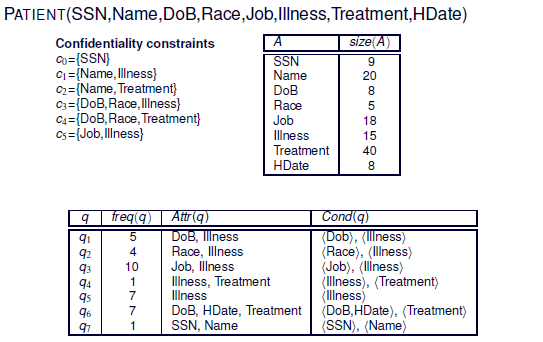
\includegraphics[scale=0.7]{img/heuristic.png}
\end{center}
\begin{center}
    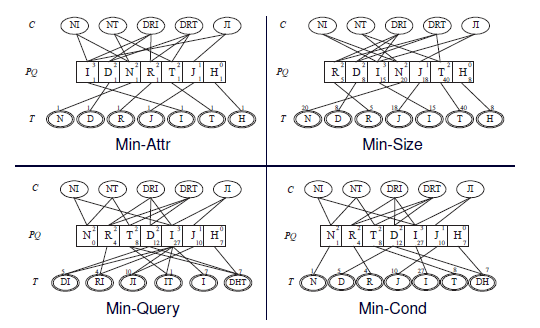
\includegraphics[scale=0.7]{img/heuristic1.png}
\end{center}
Quindi provando a esprimere questa euristica come un algoritmo:\\
\begin{itemize}
    \item \textbf{WHILE} la coda di priorità PQ ha elementi ed esiste un elemento con numero di costraint non vuoto:
    \begin{itemize}
        \item estrai l'elemento E con minore priorità data da \(\frac{E.w}{E.n_c}\)
        \item inserisci E.A in H
        \item per ogni vincolo c puntato dall'elemento E.C, rimuovi il puntatore da c ad ogni altro elemento E' nella coda e aggiorna \(E'.n_c\)
        \item per ogni target t puntato dall'elemento E.T, rimuovi il puntatore da t ad ogni altro elemento E' nella coda e aggiorna E'.w
        \item ricalcola la coda di priorità basata sui nuovi valori di priorità
    \end{itemize}
    \item \textbf{FOREACH} A \in H
    \begin{itemize}
        \item \(\frac{H}{\{A\}}\) è un hitting set per C, rimuovi A da H
    \end{itemize}
\end{itemize}

\subsubsection{Frammentazione e inferenza}
La frammentazione assume che gli attributi siano indipendenti. In presenza di dipendenza di dati abbiamo che gli attributi o le associazioni sensibili possono essere esposte indirettamente e allo stesso modo i frammenti possono essere indirettamente linkati.

\subsection{Publishing Obfuscated Associations}
Ci sono delle situazioni in cui voglio proteggere le associazioni sensibili (eventuali correlazioni), ma vorrei dare la possibilità di fare una certa query fintanto che non espongo un individuo. Ad esempio: numero medio di prodotti venduti da una farmacia senza rilevare il compratore.\\Andremo ora a vedere delle possibili soluzioni a questo problema.

\subsubsection{Anonymizing Bipartite Graph}
\begin{center}
    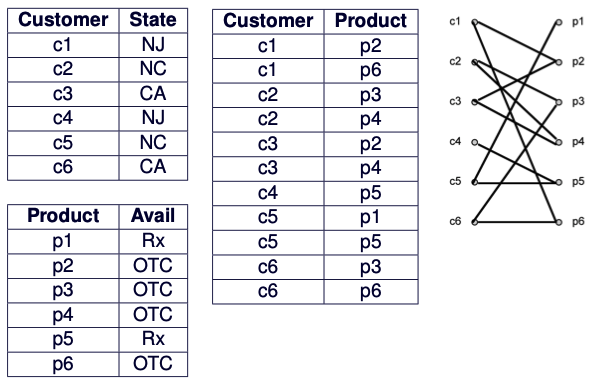
\includegraphics[scale=0.5]{img/AnonGraph.png}
\end{center}
Customer e Product le possiamo rilasciare mentre Customer-Product no, perchè è sensibile. Tuttavia vogliamo dare la possibilità di rispondere a certe query:
\begin{itemize}
    \item \textbf{Tipo 0 - Solo struttura del grafo} ad esempio il numero medio di prodotti comprati
    \item \textbf{Tipo 1 - Attributi che hanno condizioni solo da una parte del grafo} ad esempio il numero medio dei prodotti comprati da persone che vivono a Milano
    \item \textbf{Tipo 2 - Attributi che hanno condizioni da entrambe le parti del grafo} ad esempio il numero medio di prodotti X comprati da persone che vivono a Milano
\end{itemize}
\paragraph{(k,l) grouping} L'idea è quella di preservare la struttura del grafo ma permutare il mapping dalle entità ai nodi. \\
\textbf{(k,l) fa un raggruppamento di un grafo bipartito G = (V,W,E)}\\
In ciascuna delle parti del grafo bipartito creo dei gruppetti, creo degli insiemi che non si intersecano (cioè una partizione) di dimensione almeno k.\\
Prendiamo come esempio un raggruppamento (3,3) a partire dall'esempio precedente:
\begin{center}
    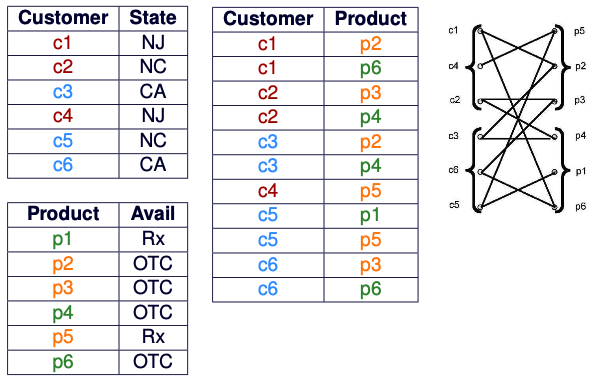
\includegraphics[scale=0.5]{img/grouping-1.png}
\end{center}
\begin{center}
    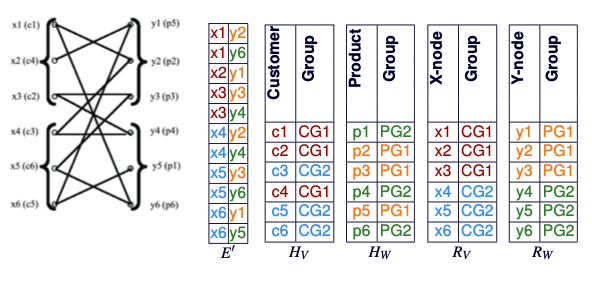
\includegraphics[scale=0.5]{img/grouping-2.png}
\end{center}
Ci sono metodi diversi per creare i raggruppamenti, ma non tutti i gruppi offrono lo stesso livello di privacy. Quello che cerchiamo di fare noi è il safe groupings: i nodi nello stesso gruppo di V non sono connessi ad uno stesso nodo in W.\\
La computazione di un raggruppamento safe può essere difficile anche per valori di k ed l piccoli.\\
Gli autori propongono un algoritmo greedy che iterativamente aggiunge un nodo a un gruppo con meno di k nodi se è safe.\\
Questo algoritmo funziona quando i grafi bipartiti sono abbastanza sparsi.

\subsubsection{Fragments and Loose Associations}
Questo metodo lavora ancora prima della frammentazione e ha come scopo quello di accrescere l'utilità del rilascio. 
Si parte sempre sapendo quali attributi (singleton) e quali associazioni sono sensibili. \\
Vengono introdotti dei requisiti di visibilità: formule booleane monotòne sugli attributi rappresentano viste sui dati (le negazioni sono gestite dai vincoli di confidenzialità), Tali requisiti permettono di esprimere differenti livelli (di requisiti) di visibilità:
\begin{itemize}
    \item attributi: alcuni attributi possono essere visibili
    \item associazioni: l'associazione tra valore di attributi dati possono essere visibili
    \item alternative views: almeno una delle viste specificate può essere visibile.
\end{itemize}
Ad esempio possiamo avere dei requisiti di visibilità sulla tabella seguente
\begin{center}
    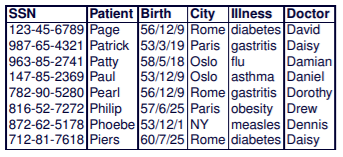
\includegraphics[scale=0.8]{img/vis1.png}
\end{center}
che ci esplicitano cosa deve essere visibile. Ad esempio:
\begin{itemize}
    \item \( Patient \lor City\)
    \item \( (Birth \land City) \lor SSN\)
    \item \( Illness \land Doctor\)
\end{itemize}
Quindi bisogna produrre delle viste che soddisfino i bisogni del cliente ma che non compromettano i vincoli di confidenzialità e che soddisfino i visibility constraints.
\begin{center}
    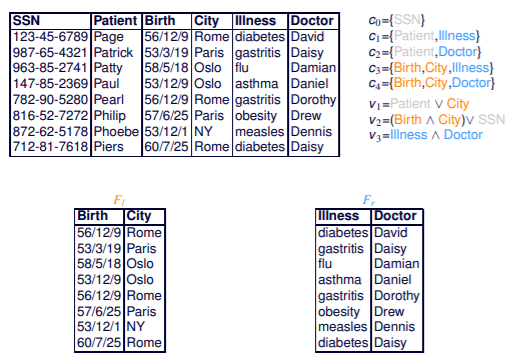
\includegraphics[scale=0.8]{img/fragex.png}
\end{center}
La frammentazione è corretta se non viola i confidentiality constraints, soddisfa i vincoli di visibilità (se chiedo di vedere le stesse cose con un AND allora le devo mettere nello stesso frammento; con un OR me ne basta una), non mi espone a correlazioni (e infatti i frammenti non hanno attributi in comune - devo anche stare attento alle dipendenze).\\
Una frammentazione corretta è minimale se il numero di frammenti è minimo (cioè ogni altra frammentazione ha un numero uguale o maggiore di frammenti). \\
Il problema Min-CF, che riguarda il calcolare una frammentazione corretta e minima, è NP-hard.\\
Un SAT-Solver può risolvere in maniera efficiente il problema Min-CF. Un'istanza del problema Min-CF è tradotta in un problema SAT. Gli input del Min-CF sono visti come formule binarie.\\
Si itera la valutazione del SAT solver, partendo da un frammento e aumentando i frammenti di uno ad ogni iterazione, fino a quando non viene trovata una soluzione (che è sicuro che sia minimale). \\
La frammentazione ovviamente rompe le associazioni tra gli attributi. Per aumentare l'utilità delle informazioni pubblicate, i frammenti possono essere accoppiati con qualche associazione in forma sanificata (deve essere garantito un grado di privacy delle associazioni).\\
Per questo vengono utilizzate \textbf{loose associations} ossia delle associazioni tra gruppi di valori.\\
Nella pratica: Ho un frammento \(F_1\) e un frammento \(F_2\). La loose association tra \(F_1\) e \(F_2\):
\begin{itemize}
    \item partiziona le tuple dei frammenti in gruppi
    \item fornisce informazioni sulle associazioni a livello di gruppo
    \item non permette la ricostruzione dell'associazione originale tra le tuple nel frammento
    \item fornisce un'utilità arricchita dei dati pubblicati
\end{itemize}
Quindi si pubblica a livello di gruppo (invece nel metodo Anonymizing Bipartite Graph si faceva aliasing). \\
Come funziona il k-grouping: vado a raggruppare le tuple in gruppetti che siano grandi almeno k. Un k-grouping fatto su un certo frammento è minimale se massimizza il numero di gruppi. Raggruppo in \(k_1\) e \(k_2\). Un raggruppamento (\(k_1\), \(k_1\)) è minimale se da entrambe le parti si è fatto un raggruppamento minimale.\\
\begin{center}
    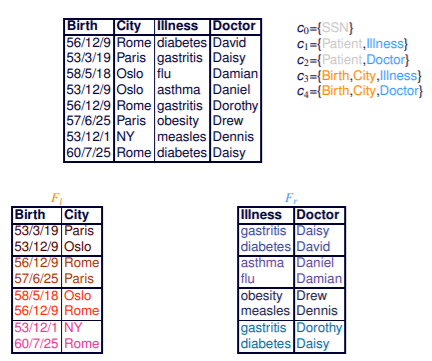
\includegraphics[scale=0.7]{img/Mingroup1.png}
\end{center}
Un raggruppamento (\(k_l\), \(k_r\)) introduce un'associazione di gruppo A tra i gruppi in \(f_l\) e \(f_r\). \\
Un'associazione di gruppo A tra i due frammenti \(f_l\) e \(f_r\) è una coppia di gruppi di identificatori tali che:
\begin{itemize}
    \item A ha la stessa cardinalità della relazione originale
    \item c'è un mapping biettivo tra la relazione originale e A che associa ogni tupla nella relazione originale con una coppia (\(G_l(l)\),\(G_r(r)\)) in A, con \(l \in f_l\) e \(r \in f_r\)
\end{itemize}
\begin{center}
    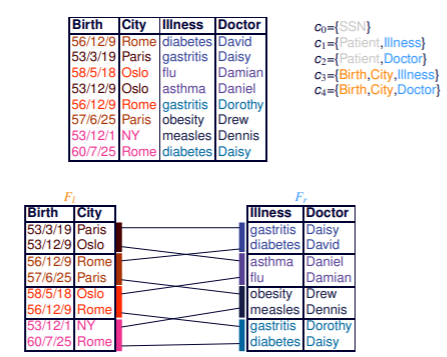
\includegraphics[scale=0.8]{img/groupass1.png}
\end{center}
Pubblichiamo le associazioni a livello di gruppo e non a livello della singola tupla e il risultato è il seguente:
\begin{center}
    \includegraphics[scale=0.8]{img/groupass2.png}
\end{center}
La pubblicazione dei gruppi è fatta in modo loose, quindi aumento l'incertezza di \\ 2 x 2 = 4 (ad ogni elemento potrebbero corrisponderne 4).\\
I duplicati nei frammenti vengono mantenuti (siccome tutti i frammenti hanno la stessa cardinalità della relazione originale) e quindi potrebbero contenere tuple uguali.\\
Anche delle tuple diverse potrebbero avere stessi valori per gli attributi coinvolti nei vincoli di confidenzialità. La protezione looseness offerta dal raggruppamento potrebbe quindi essere compromessa: dobbiamo controllare le occorenze degli stessi valori.\\
Due tuple sono simili (alike \(\simeq\)) rispetto ad un vincolo c se:
\begin{itemize}
    \item il vincolo c è coperto dall'unione (inteso come unione di attributi) dei due frammenti \(F_r\) e \(F_l\)
    \item una tupla che si interseca con i vincoli è uguale all'altra tupla che si interseca con i vincoli
\end{itemize}
Questa proprietà di somiglianza è transitiva per ciascun vincolo c.\\
Non è transitiva invece se ci sono almeno due vincoli coperti da \(F_r\) e \(F_l\)
\begin{center}
    \includegraphics[scale=0.8]{img/alikeness.png}
\end{center}
Un'associazione a livello di gruppo è k-loose se ogni tupla in un gruppo può corrispondere dall’altra parte ad almeno k associazioni diverse. Proprietà: se sei k-loose su 4 allora sei k-loose anche su 3, su 2, ... \\
Un'associazione di gruppo A è minimale su (\(k_l\), \(k_r\)) se:
\begin{itemize}
    \item A è k-loose
    \item non era possibile fare di meglio (cioè non c’era un’altra associazione con valori più piccoli che dava lo stesso grado di loose).
\end{itemize}
Se vogliamo garantirci un'associazione k-loose allora tale associazione a livello di gruppo deve tocare tuple che sono diverse e non sono simili.\\
Se un raggruppamento (\(k_l\), \(k_r\)) soddisfa le seguenti proprietà di eterogeneità:
\begin{itemize}
    \item di gruppo: nessun gruppo può contenere tuple che sono simili rispetto a qualche vincolo
    \item di associazione: nessun gruppo può essere associato due volte con lo stesso gruppo, altrimenti perderei l'incertezza
    \item profonda: nessun gruppo può essere associato con due gruppi che hanno tuple simili
\end{itemize}
allora l'associazione tra i gruppi è k-loose con k=\(k_l\) x \(k_r\). \\
Un raggruppamento (\(k_l\), \(k_r\)) è:
\begin{itemize}
    \item flat se almeno uno tra \(k_l\) e \(k_r\) sono uguali a 1. In questo caso assomiglia a k-anonimity e l-diversity insieme, ma lavora sulle associazioni e i valori degli attributi non sono generalizzati
    \begin{center}
        \includegraphics[scale=0.5]{img/flat.png}
    \end{center}
    \item sparse se sia \(k_l\) che \(k_r\) sono diversi da 1. Garantisce una larga applicabilità rispetto al raggruppamento flat, con lo stesso livello di protezione
    \begin{center}
        \includegraphics[scale=0.5]{img/sparse.png}
    \end{center}
\end{itemize}
La pubblicazione di associazioni loose incrementa l'utilità dei dati poichè rende possibile la valutazione di query in modo più preciso rispetto alla  pubblicazione dei soli frammenti. Questo però comporta ad un'esposizione delle informazioni (grado di privacy più basso).\\
L'esposizione di un'associazione sensibile \(\langle l[c \cap F_l],r[c \cap F_r] \rangle\) con c che è un vincolo coperto da \(F_l\) e \(F_r\) può essere espressa come la probabilità che ci sia quell'associazione nella relazione originale.\\
L'incremento di esposizione derivata dalla pubblicazione di un'associazione loose può essere misurata come la differenza tra:
\begin{itemize}
    \item la probabilità \(P^A(l[c \cap F_l],r[c \cap F_r])\) che l'associazione sensibile \(\langle l[c \cap F_l],r[c \cap F_r] \rangle\) compaia nella relazione originale dati \(f_l, f_r\) e A
    \item la probabilità \(P(l[c \cap F_l],r[c \cap F_r])\) che l'associazione sensibile \(\langle l[c \cap F_l],r[c \cap F_r] \rangle\) compaia nella relazione originale dati \(f_l\) e \(f_r\)
\end{itemize}
Dati \( l \in f_l\) e \(r \in f_r\) la probabilità P(l,r) che la tupla \(\langlel,r\rangle\) appartenga alla relazione originale è \( \frac{1}{|f_l|} = \frac{1}{|f_r|}\)
\begin{center}
    \includegraphics[scale=0.5]{img/exposure.png}
\end{center}
L'esposizione di (P(\(l[c \cap F_l],r[c \cap F_r]\))) dipende dalla presenza di tuple simili. Siano \(l_i,l_j\) due tuple in \(f_l\) tali che \(l_i \simeq_c l_j\), P(\(l_i[c \cap F_l],r[c \cap F_r]\)) è la composizione delle probabilità che:
\begin{itemize}
    \item \(l_i\) sia associato con r
    \item \(l_j\) sia associato con r
\end{itemize}
\[ P(l_i,r) + P(l_j,r) - (P(l_i,r) * P(l_j,r))\]

Dalla tabella precedente (considerando il vincolo 3 = {Birth, City, Illness}) dobbiamo togliere le tuple simili che mi fanno diventare la tabella come segue (abbiamo usato la formula definita precedentemente di combinazione di probabilità): 
\begin{center}
    \includegraphics[scale=0.5]{img/exposure1.png}
\end{center}
Questo si verifica nel caso in cui si decidesse di non pubblicare le associazioni loose.\\
Nel caso contrario invece si partirebbe da una situazione simile a quella seguente:
\begin{center}
    \includegraphics[scale=0.5]{img/exposure2.png}
\end{center}
Dati \(l \in f_l\) e \(r \in f_r\) la probabilità \(P^A(l,r)\) che la tupla \(\langle l,r \rangle\) appartiene alla relazione originale è almeno \(\frac{1}{k}\).\\
\(P^A(l[c \cap F_l],r[c \cap F_r])\) è valutata considerando la somiglianza. Siano \(l_i,l_j\) due tuple in \(f_l\) tali che \(l_i \simeq_c l_j\), \(P^A(l_i[c \cap F_l],r[c \cap F_r])\) è la composizione delle probabilità che:
\begin{itemize}
    \item \(l_i\) sia associato con r
    \item \(l_j\) sia associato con r
\end{itemize}
\[ P^A(l_i,r) + P^A(l_j,r) - (P^A(l_i,r) * P^A(l_j,r))\]
Applichiamo lo stesso procedimento visto in precedenza e otterremo:
\begin{center}
    \includegraphics[scale=0.5]{img/exposure3.png}
\end{center}
Abbiamo parlato di utilità e privacy dei dati. Come possiamo misurarle?
\begin{itemize}
    \item \textbf{utilità}: media delle differenze di probabilità delle due tabelle (con associazioni e senza associazioni) per ogni associazione sensibile
    \item \textbf{privacy}: data una soglia di privacy verifico che la differenza sopra citata non vada mai a superarla
\end{itemize}